\vspace{10pt}

{\centering\subsection*{刘笑:我学会了洗碗}}

\addcontentsline{toc}{subsection}{刘笑:我学会了洗碗}

\renewcommand{\leftmark}{刘笑:我学会了洗碗}

\begin{figure}[htbp]

\centering

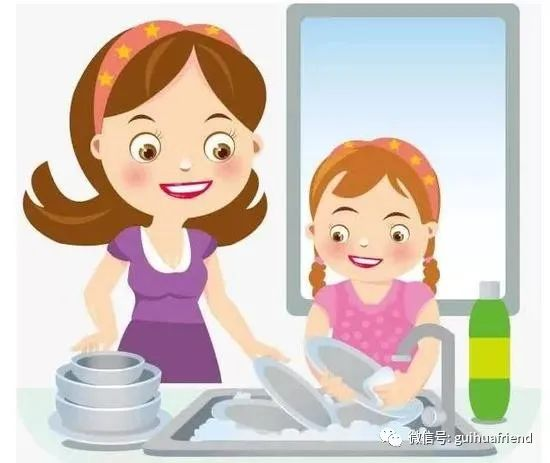
\includegraphics[width = .5\textwidth]{./ch/4.jpg}

\end{figure}





今天我决定要尝试着自己洗碗,中午我们一家吃完饭,我跑到妈妈面前说:“妈妈,今天我来帮你洗碗。”妈妈可高兴坏了,笑眯眯地说:“好啊,不过你会洗碗吗?”我对妈妈说:“不会啊!你在旁边教教我。”

妈妈帮我系上了围裙。准备好洗碗了,我按照妈妈的方法去做,先把水接满,再把碗放进去。我学妈妈一样在里面加了一些洗洁精,结果洗洁精挤多了,挤得到处都是。第一只碗我没洗干净,碗里有很多泡沫。我心想:我怎么这么笨啊?都不会洗碗。妈妈走到我面前,鼓励我说:“不用灰心,多试几次你一定会成功的。”

第二次洗碗时,这次我认真的把碗洗干净了,但把碗拿出来时摔破了,我本来想放弃的,可我想:妈妈既然会洗碗,我也一定能学会,不能让他失望。第三次,妈妈开始一步一步的教我。这次既没挤多洗洁精,也没把碗摔破,而是把碗洗的闪闪发光,晶莹剔透。

通过这件事我懂得了,无论做什么事情都要有耐心?而且我还知道了父母们平时有多么的辛苦。





\vspace{10pt}



作者:四(2)班 刘笑



指导老师:陈小丽



投稿:2021年6月11日



发表:2021年6月15日






                



\vspace{10pt}

\hline



